\documentclass[11pt]{article}
\usepackage[review]{acl}
\usepackage{times}
\usepackage{latexsym}
\usepackage[T1]{fontenc}
\usepackage[utf8]{inputenc}
\usepackage{microtype}
\usepackage{inconsolata}
\usepackage{graphicx}
\graphicspath{{../../artifacts/figures/}}
\usepackage{amsmath}
\usepackage{amssymb}
\usepackage{amsthm}
\usepackage{algorithm}
\usepackage{algorithmic}
\usepackage{booktabs}
\usepackage{multirow}
\usepackage{enumitem}
\usepackage{tikz}
\usetikzlibrary{positioning,arrows.meta}
\newtheorem{proposition}{Proposition}
\newtheorem{definition}{Definition}

\newcommand{\bstar}{b^*}
\newcommand{\aeff}{\alpha_{\mathrm{eff}}}
\newcommand{\nmin}{n_{\min}}
\newcommand{\btau}{b_{\tau}}
\newcommand{\bess}{b_{\mathrm{ESS}}}
\setlength{\textfloatsep}{6pt plus 2pt minus 2pt}
\setlength{\floatsep}{6pt plus 2pt minus 2pt}
\setlength{\abovecaptionskip}{4pt plus 1pt minus 1pt}
\setlength{\belowcaptionskip}{0pt}
\title{When Does Detect-and-Reweight Work for Synthetic Contamination?}

\author{Anonymous}

\begin{document}
\maketitle

\begin{abstract}
As synthetic text pervades web corpora, detect-and-reweight methods that downweight likely-synthetic samples during training have emerged to prevent model collapse, yet when they actually help remains unclear.
We investigate this question through controlled continued-pretraining experiments (Qwen3-0.6B, 132M tokens, 5 seeds) and identify three effectiveness conditions.
First, detect-and-remove (D\&R) outperforms all reweighting methods in our setting; epoch-matched controls attribute over 95\% of the advantage to multi-epoch exposure on filtered data, identifying the mechanism behind D\&R's effectiveness.
Second, the detector must provide both sufficient discrimination \emph{and} good calibration; high-AUC detectors with poor calibration degrade performance below uniform training.
Third, minimum intervention, applying the smallest reweighting exponent that meets a quality floor, outperforms unconstrained weight maximization.
As an illustrative application of the minimum-intervention principle, we derive a dual-constrained adaptive exponent $\bstar$ that improves over uniform training at contamination ratios $\rho \geq 0.4$, reaching conventional significance after multiple-comparison correction, while requiring no per-model tuning.
These findings apply within our self-contamination setup at 0.6B scale; generalization to cross-model contamination and larger models remains to be established\footnote{Code and data are available at \url{https://anonymous.4open.science/r/provenance_weight_training-F72D/}.}.

\end{abstract}

\section{Introduction}
\label{sec:intro}
The detect-and-reweight paradigm~\citep{drayson2025detection} has emerged as a response to synthetic contamination in web corpora, now estimated at 20--60\% of crawled data~\citep{cheng2025contamination}.
Training on such data risks model collapse~\citep{shumailov2024model,dohmatob2025strong}, motivating methods that downweight likely-synthetic samples via $w(x) = (1 - q(x))^b$, where $q(x)$ is a detector's synthetic probability and $b$ is a sharpening exponent.
An alternative, Detect and Remove (D\&R), hard-filters samples above a threshold~\citep{feng2025beyond}.

\begin{figure*}[t]
\centering
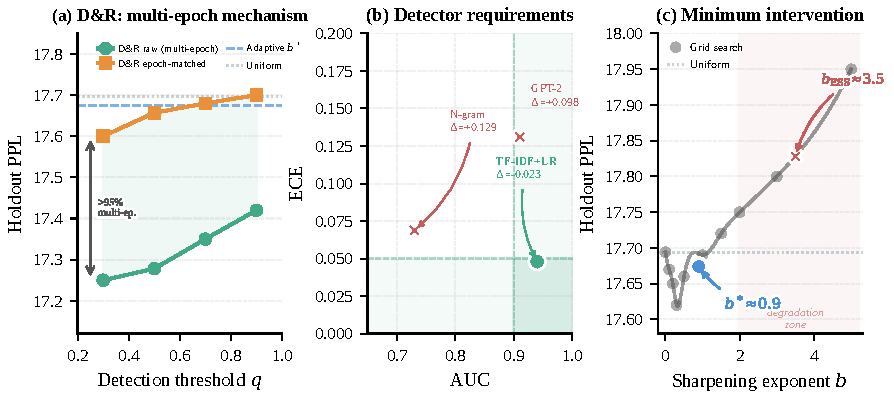
\includegraphics[width=\textwidth]{fig1_overview}
\caption{Three effectiveness conditions for detect-and-reweight.
\textbf{(a)}~D\&R achieves the best raw perplexity (PPL); epoch-matched controls reveal that multi-epoch exposure on filtered data accounts for the bulk of the advantage (\S\ref{sec:results}).
\textbf{(b)}~Only detectors with both high AUC \emph{and} low ECE fall in the effective zone; comparable AUC with poor calibration degrades PPL below uniform.
\textbf{(c)}~Adaptive $\bstar{\approx}0.9$ operates near the grid-search optimum, while ESS-only $b{\approx}3.5$ falls in the degradation zone.}
\label{fig:overview}
\end{figure*}

Despite growing adoption, the paradigm's effectiveness conditions are poorly characterized.
What mechanism drives D\&R's strong performance, and how does it compare to soft reweighting under controlled conditions?
What detector properties are necessary for effective reweighting?
How does the reweighting mechanism behave across contamination levels, and can $b$ be set without per-model grid search?

We investigate these questions through controlled experiments on Qwen3-0.6B continued pretraining (132M FineWeb tokens, $\rho{=}0.4$, 5 seeds), with extensions to $\rho \in \{0.2, 0.6\}$ and 1.7B parameters (\S\ref{sec:limitations} discusses scope).
To ground the analysis of exponent selection, we implement a dual-constrained formulation as an illustrative application: find the minimum $b$ such that $\aeff(b) \geq \tau$ (quality floor, motivated by convergence theory~\citep{wang2026survive}), subject to $\mathrm{ESS}(b) \geq \nmin$ (stability ceiling)~\citep{kish1965survey,vehtari2024psis}.

Our analysis yields three findings:
\begin{itemize}[nosep,leftmargin=*]
\item \textbf{D\&R as the strongest strategy.}
D\&R outperforms all reweighting methods in our setting (PPL $17.250$ vs.\ $17.674$, 3 seeds); epoch-matched controls attribute ${>}$95\% of the advantage to multi-epoch exposure on filtered data, reducing the gap to $\Delta{=}0.017$ (Table~\ref{tab:epoch_match}).

\item \textbf{Detector requirements for effective reweighting.}
Both sufficient discrimination (area under the ROC curve; AUC) and good calibration (expected calibration error; ECE) are empirically observed requirements in our self-contamination setting; a high-AUC but poorly calibrated detector degrades performance below uniform (3 detectors, 3 seeds; \S\ref{sec:robustness}).

\item \textbf{Minimum intervention outperforms maximization.}
An $\aeff$ quality constraint binds in ${\sim}$50\% of batches at ${\approx}4{\times}$ lower sharpening exponents than an ESS-only alternative (\S\ref{sec:regime}); at $\rho{=}0.6$, ESS-only collapses toward uniform while the dual constraint maintains its advantage.
\end{itemize}
To demonstrate the minimum-intervention principle, we derive a dual-constrained adaptive $\bstar$ that eliminates per-model grid search ($\Delta{=}{-}0.023$ at $\rho{=}0.4$, $-$0.032 at $\rho{=}0.6$; Table~\ref{tab:main}), with transferable defaults ($\tau{=}0.7$, $\nmin{=}\lfloor B/2 \rfloor$).
The method fails at $\rho{=}0.2$; at 1.7B it shows no degradation but the benefit diminishes.


\section{Related Work}
\label{sec:related}
\paragraph{Synthetic Contamination and Model Collapse.}
Training on recursively generated data leads to irreversible quality degradation (\emph{model collapse})~\citep{shumailov2024model}.
\citet{alemohammad2024mad} formalize this as Model Autophagy Disorder, showing that quality inevitably degrades without fresh real data.
More critically, \citet{dohmatob2025strong} prove under scaling-law regimes that even a vanishingly small synthetic fraction suffices to trigger collapse, ruling out data scaling as a remedy.
\citet{cheng2025contamination} confirm that synthetic content now constitutes an estimated 20--60\% of web corpora, though accumulating real data avoids divergence~\citep{kazdan2025collapse} and even minimal curation suffices~\citep{amin2025escaping}.
Not all synthetic data is harmful: the Phi series~\citep{gunasekar2023textbooks,li2023textbooks2} demonstrates that curated synthetic data can improve training efficiency, but this assumes intentional generation with quality control, unlike the uncontrolled web contamination we address.

\paragraph{Detection, Filtering, and Data Reweighting.}
Continuous-score detectors---probability curvature~\citep{mitchell2023detectgpt}, cross-perplexity ratios~\citep{hans2024binoculars}, low-probability token statistics~\citep{shi2024minkprob}---enable document-level weighting~\citep{wu2025survey}.
Data composition is optimized via perplexity filtering~\citep{wenzek2020ccnet}, domain-level importance sampling~\citep{xie2023doremi,xie2023dsir,grangier2025crisp,ye2025mixing}, instance-level strategies~\citep{bengio2009curriculum,mindermann2022prioritized,sow2025dynamic,engstrom2024dsdm}, and deduplication~\citep{abbas2023semdedup}; see \citet{albalak2024survey}.
None targets synthetic provenance; moreover, classifier-based quality scores may capture stylistic similarity rather than intrinsic quality~\citep{naitsaada2025illusion}.
Most directly related, \citet{drayson2025detection} propose $w_j = (1{-}q_j)^b$ for collapse prevention via detect-and-reweight in from-scratch pretraining, where $q_j$ is the detector's synthetic probability. We adopt the same formula but differ fundamentally:
\textbf{(i)}~Drayson et al.\ select $b$ via validation-set grid search, with different model scales requiring different values ($b{=}10$ for ${\leq}360$M, $b{=}1$ for 1.7B); our $\bstar$ is derived per-batch from dual constraints ($\aeff \geq \tau$, $\mathrm{ESS} \geq \nmin$) at zero validation cost.
\textbf{(ii)}~Their sampling importance resampling (SIR) discretizes the weight distribution; we apply direct loss reweighting with continuous gradients.
\textbf{(iii)}~They employ a ModernBERT-150M detector (AUC\,=\,0.986) on WikiText-2 (${\sim}$2M tokens); we show that a lightweight TF-IDF + logistic regression detector (AUC\,=\,0.94) suffices on FineWeb-scale data (132M+ tokens), and both calibration and sufficient discrimination appear required for effective reweighting.

\paragraph{Theoretical Foundations.}
Importance weighting theory underpins our constraints. \citet{cortes2010learning} establish generalization bounds governed by the weight second moment, directly motivating our ESS floor since $\mathrm{ESS} = n/\mathbb{E}[w^2]$.
\citet{fang2020rethinking} show that na\"ive importance weighting degrades in deep networks under distribution shift, motivating adaptive, bounded schemes such as ours.
For LLM pretraining, \citet{sow2025dynamic} prove convergence guarantees for instance-level reweighting under bounded weight variance---a condition our ESS constraint explicitly enforces---while \citet{ye2025mixing} derive functional laws governing how mixture proportions affect loss, complementing our instance-level approach.
\citet{he2025golden} derive the optimal real-data weight under known mixture proportions (the golden-ratio reciprocal ${\approx}0.62$); their result requires the contamination ratio $k$, unavailable in web-scale settings, so we use it as an oracle baseline.
\citet{wang2026survive} prove that contaminated recursive training converges at a rate governed by the effective real-data fraction $\alpha$; this motivates our quality threshold $\aeff(b) \geq \tau$.
We operationalize this without the known-proportion assumption, estimating $\aeff$ from batch-level statistics online.
Score calibration~\citep{guo2017calibration} is relevant because miscalibration systematically biases $\aeff$; for the stability constraint, we build on Kish's effective sample size~\citep{kish1965survey}.


\section{Method}
\label{sec:method}
\begin{figure}[t]
\centering
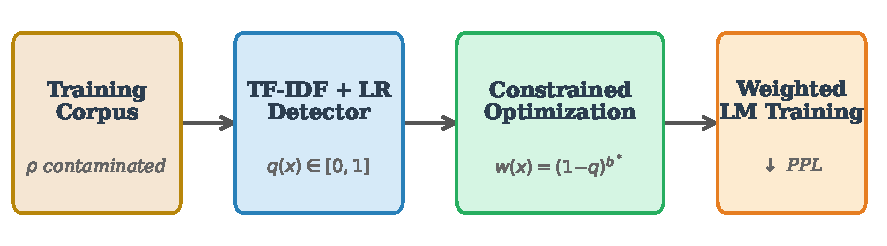
\includegraphics[width=\columnwidth]{dr_pipeline_concept}
\caption{Overview of the detect-and-reweight pipeline. A TF-IDF + LR detector assigns contamination scores $q(x)$; a dual-constrained optimizer selects $b$ to satisfy quality-floor and effective-sample-size constraints; the resulting weights $w(x) = (1{-}q(x))^{b}$ are applied during training.}
\label{fig:pipeline}
\end{figure}

Figure~\ref{fig:pipeline} illustrates the pipeline. Let $\mathcal{D}$ denote a pretraining corpus with unknown synthetic contamination ratio $\rho$~\citep{cheng2025contamination}.
A detector assigns each sample $x$ a synthetic probability $q(x) \in [0,1]$; following \citet{drayson2025detection}, we weight each sample as $w(x) = (1 - q(x))^{b}$, where $b \geq 0$ is a sharpening exponent ($b{=}0$ recovers uniform training).
Rather than selecting $b$ via grid search, we derive $b$ per-batch from the batch's $q$-score distribution using two opposing constraints.

Given a batch $\mathcal{B} = \{x_1, \ldots, x_B\}$ with scores $q_i = q(x_i)$ and weights $w_i(b) = (1 - q_i)^{b}$:

\paragraph{Quality floor.}
The \emph{effective authenticity} $\aeff(b) = \sum_i w_i(b)(1{-}q_i) / \sum_i w_i(b)$ measures the weighted mean detector confidence that samples are real.
We require $\aeff(b) \geq \tau$, yielding a lower bound $b_\tau$ on the exponent, motivated by convergence theory under contamination~\citep{wang2026survive}.
$\aeff$ correlates with the true batch-level real fraction at Pearson $r \approx 0.79$ (Appendix~\ref{app:alpha_validation}); limitations are discussed in \S\ref{sec:discussion}.

\paragraph{Stability ceiling.}
Kish's effective sample size $\mathrm{ESS}(b) = (\sum_i w_i)^2 / \sum_i w_i^2$~\citep{kish1965survey} decreases monotonically in $b$ (Appendix~\ref{app:proofs}).
We require $\mathrm{ESS}(b) \geq \nmin$, yielding an upper bound $\bess$.

\paragraph{Adaptive $\bstar$.}
Since $\aeff$ is non-decreasing and ESS is decreasing in $b$, the two constraints define an interval $[b_\tau, \bess]$.
The optimal exponent implements \emph{minimum intervention}:
\begin{equation}
  b^{*} = \begin{cases}
    0        & \text{if } \aeff(0) \geq \tau, \\
    b_\tau   & \text{if } b_\tau \leq \bess, \\
    \bess & \text{otherwise (stability precedence)},
  \end{cases}
  \label{eq:bstar}
\end{equation}
applying the smallest $b$ that achieves the quality floor.
Each batch falls into one of three regimes (clean, $\aeff$-binding, or ESS-binding; Figure~\ref{fig:dual_constraint}) whose frequencies we analyze in \S\ref{sec:regime}.
The resulting $\bstar$ trajectory (Figure~\ref{fig:bstar_traj}, Appendix) varies substantially across batches, with all three regimes alternating throughout; this per-batch variation indicates adaptation to local composition rather than global dynamics.

\begin{figure*}[t]
\centering
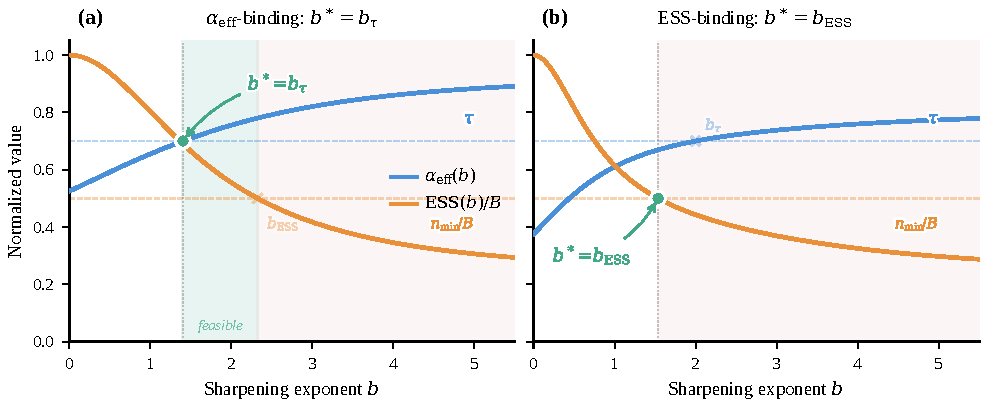
\includegraphics[width=\textwidth]{dual_constraint_illustration}
\caption{Dual-constraint $\bstar$ selection for two representative batches ($B{=}4$, $\tau{=}0.7$, $\nmin{=}2$).
\textbf{(a)}~Quality constraint binds: $\aeff(b)$ reaches $\tau$ before $\mathrm{ESS}(b)$ drops below $\nmin$, so $\bstar = \btau$.
\textbf{(b)}~Stability constraint binds: $\mathrm{ESS}(b)$ hits the floor first, so $\bstar = \bess$.
Green: feasible interval; red: over-sharpening.}
\label{fig:dual_constraint}
\end{figure*}

Given $\bstar$, normalized weights $\pi_i = w_i(\bstar) / \sum_j w_j(\bstar)$ define the weighted loss $\mathcal{L} = \sum_i \pi_i \ell_i$; $\bstar$ is found via bisection (Algorithm~\ref{alg:bstar}, Appendix~\ref{app:algorithm}) in $\mathcal{O}(B \log(b_{\max}/\varepsilon))$ operations, negligible beside the forward pass.
Defaults: $\tau{=}0.7$, $\nmin{=}\lfloor B/2 \rfloor$; sensitivity in \S\ref{sec:sensitivity}.



\section{Experimental Setup}
\label{sec:experiments}
\paragraph{Training Data.}
We sample a 132M-token subset of FineWeb~\citep{penedo2024fineweb} as the real-data source, comparable to typical domain-adaptive continued pretraining budgets~\citep{gururangan2020dont}.
To simulate web-scale synthetic contamination, we generate continuations with Qwen3-0.6B~\citep{yang2025qwen3}, the same architecture used for continued pretraining, and inject them at token-level ratio $\rho = 0.4$ via uniform random mixing.\footnote{$\rho$ denotes the token-level contamination ratio. Because synthetic documents are shorter on average (304 vs.\ 560 words), the document-level synthetic fraction is 55.6\% at $\rho{=}0.4$.}
This self-contamination design means generator and trainee share the same distribution, providing a controlled testbed with known ground-truth labels but limiting ecological validity; cross-model transfer results (Appendix~\ref{app:cross_model}) are mixed, and we discuss implications for detection difficulty in \S\ref{sec:limitations}.

\paragraph{Detector.}
We train a TF-IDF + Logistic Regression classifier on a held-out labeled split (AUC\,=\,0.94, calibrated ECE\,=\,0.048 after temperature scaling with $T{=}0.204$).
The resulting $q$-scores have mean 0.60, standard deviation 0.37, and median 0.71, with 46.3\% of samples in the uncertain range $[0.2, 0.8]$.
We use this lightweight detector rather than neural alternatives (e.g., ModernBERT at AUC\,${\geq}$\,0.98 in \citealt{drayson2025detection}) to test whether score \emph{calibration} may matter as much as raw discrimination for reweighting.
To evaluate detector sensitivity, we additionally test two generative baselines: a GPT-2-based perplexity scorer (AUC\,=\,0.91) and an N-gram language model perplexity scorer (AUC\,=\,0.73); results are reported in \S\ref{sec:robustness} (implementation details in Appendix~\ref{app:detector_details}).

\paragraph{Training.}
Table~\ref{tab:config} summarizes the training configuration.
We use $B{=}4$ as the default micro-batch size, reflecting memory constraints typical of continued pretraining setups; \S\ref{sec:sensitivity} demonstrates that larger batches amplify the adaptive advantage.
All main comparisons use three random seeds (42, 123, 456) trained from scratch (Appendix~\ref{app:resume_artifact}); the primary comparison is extended to five seeds (adding 789, 234).

\begin{table}[t]
\centering
\small
\begin{tabular}{@{}ll@{\hspace{8pt}}ll@{}}
\toprule
Model & Qwen3-0.6B & Optimizer & AdamW \\
Steps & 6{,}103 & Peak LR & $5{\times}10^{-5}$ \\
Micro-batch & $B{=}4$ & Schedule & linear + warmup \\
Grad.\ accum. & 4 ($B_{\mathrm{eff}}{=}16$) & Seq.\ len. & 2048 \\
Precision & bf16 & GPU & 1$\times$ RTX PRO 6000 \\
\bottomrule
\end{tabular}
\caption{Training configuration for continued pretraining.}
\label{tab:config}
\end{table}

\paragraph{Evaluation.}
We report held-out perplexity (PPL) on 5{,}000 documents from a FineWeb holdout set ($\sim$4M tokens) containing only human-authored text, via sliding-window evaluation (stride 1024).
All evaluations are post-hoc with a unified pipeline; training involves no inline evaluation.

\paragraph{Methods.}
We compare six approaches:
\begin{itemize}[nosep,leftmargin=*]
  \item \textbf{Uniform}: $w_j = 1$ for all $j$ (no contamination handling).
  \item \textbf{Grid-$b$}: fixed $b \in \{0.1, 0.2, 0.3, 0.5, 1.0, 1.5, 2.0, 3.0, 5.0\}$ (nine candidates), best selected post-hoc by held-out PPL.
        Represents validation-based selection~\citep{drayson2025detection}.
  \item \textbf{ESS-only}: $\bstar = \max\{b : \mathrm{ESS}(b) \geq \nmin\}$, the maximum-intervention variant retaining only the stability constraint, ablating $\aeff$.
  \item \textbf{Golden Ratio}: $w = 1/\varphi \approx 0.618$ for synthetic ($q_j > 0.5$), $w = 1$ otherwise~\citep{he2025golden}.
        Requires known provenance labels (oracle).
  \item \textbf{Adaptive} (ours): per-batch $\bstar$ from the dual-constraint formulation (\S\ref{sec:method}), with $\tau = 0.7$ (default; $\tau{=}0.8$ comparable, \S\ref{sec:sensitivity}) and $\nmin = 2$ (half the micro-batch size).
  \item \textbf{Detect \& Remove}: hard filtering that discards samples with $q_j > 0.5$ and trains uniformly on the remainder.
        Requires a calibrated detection threshold; threshold sensitivity is analyzed in \S\ref{sec:main-results}.
\end{itemize}


\section{Results}
\label{sec:results}
\begin{table}[t]
\centering
\small
\setlength{\tabcolsep}{3pt}
\resizebox{\columnwidth}{!}{%
\begin{tabular}{@{}lcccc@{}}
\toprule
\textbf{Method} & \textbf{Seed 42} & \textbf{Seed 123} & \textbf{Seed 456} & \textbf{Mean} \\
\midrule
Uniform                & 17.694 & 17.686 & 17.702 & 17.697 $\pm$ .008 \\
Adaptive $\bstar$ (ours) & \textbf{17.680} & \textbf{17.666} & \textbf{17.677} & \textbf{17.674} $\pm$ .006 \\
ESS-only               & 17.730 & 17.720 & 17.760 & 17.737 $\pm$ .021 \\
Random $\mathcal{U}(0,2)$ & 17.830 & 17.800 & 17.777 & 17.802 $\pm$ .027 \\
Permuted $q$-scores  & 17.919 & --     & --     & 17.919 \\
\bottomrule
\end{tabular}}
\caption{Main comparison: held-out PPL ($\downarrow$) at $\rho{=}0.4$, 1 content epoch.
Adaptive and Uniform: 5-seed means (seeds 42, 123, 456, 789, 234); ESS-only and Random: 3-seed means (seeds 42, 123, 456); Permuted: single seed (42).
Adaptive uses $\tau{=}0.7$, $\nmin{=}2$.
Permuted randomly shuffles $q$-scores across samples, destroying provenance signal while preserving weight non-uniformity ($\Delta{=}{+}0.225$).}
\label{tab:main}
\end{table}

\subsection{Main Results}
\label{sec:main-results}

Table~\ref{tab:main} reports held-out perplexity at $\rho = 0.4$ across five seeds.
Continued pretraining reduces PPL from 22.970 to the 17.3--17.8 range; method comparisons operate within a narrow residual.

Adaptive $\bstar$ achieves 5-seed mean PPL 17.674, compared to 17.697 for uniform ($\Delta{=}{-}0.023$, directionally consistent across all seeds) and 17.620 for grid $b{=}0.3$ (3-seed mean, post-hoc oracle; gap $+$0.054; Table~\ref{tab:aux}).
A paired $t$-test yields $t(4){=}{-}8.21$, $p{=}0.0012$; after Bonferroni--Holm correction for nine family-wise comparisons, $p_{\mathrm{BH}}{=}0.011$, reaching conventional significance at $\alpha{=}0.05$.
The engineering benefit is eliminating $b$ grid search (nine full training runs~\citep{drayson2025detection}, ${\sim}$16 GPU-hours at 0.6B scale, scaling linearly with model size), though grid search yields a larger improvement.
The grid-best $b{=}0.3$ is a post-hoc oracle from nine candidates with ${\sim}6{\times}$ higher cross-seed standard deviation than adaptive ($\sigma{=}0.035$ vs.\ $0.006$); the noisy PPL plateau at $b \in [0.1, 0.5]$ (Figure~\ref{fig:grid_b_trend}) makes validation-based selection unreliable.
At the nearest fixed point ($b{=}1.0$), PPL equals uniform (17.692 vs.\ 17.694): per-batch adaptation is essential.

The ablation hierarchy at $\rho{=}0.4$ (Adaptive ${<}$ Uniform ${<}$ ESS-only ${<}$ Random ${<}$ Permuted, Table~\ref{tab:main}) reveals two requirements for effective reweighting: detector signal and minimum intervention.
Random weights $\mathcal{U}(0,2)$ (17.802) confirm that non-uniform weighting alone does not help; permuted $q$-scores (17.919, $\Delta{=}{+}0.225$) further isolate provenance signal as load-bearing, since shuffling destroys the detector's sample-level information while preserving identical weight non-uniformity.
ESS-only (mean $17.737 {\pm} 0.021$) uses the same $q$-scores but maximizes $b$ up to the stability ceiling, concentrating weights on a few high-confidence samples; it degrades PPL by 0.043 relative to uniform.
Only the dual-constrained adaptive method, which limits $b$ to the minimum needed, improves in-distribution PPL over uniform (mean $\Delta{=}{-}0.023$, directionally consistent across all seeds).
Figure~\ref{fig:grid_b_trend} contextualizes both results: adaptive $\bstar$ operates near the curve minimum while ESS-only $\bstar$ (mean ${\approx}$3.5) falls in the degradation zone.

\begin{figure}[t]
\centering
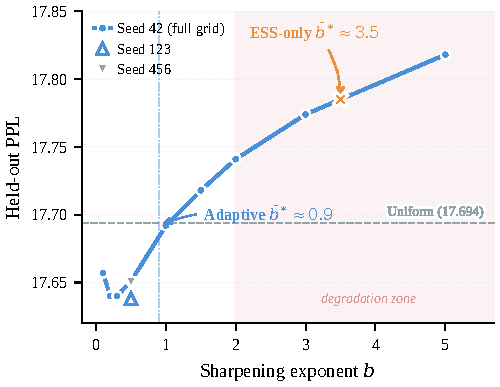
\includegraphics[width=\columnwidth]{grid_b_trend_clean}
\caption{Held-out PPL as a function of fixed sharpening exponent $b$ (grid search, $\rho{=}0.4$).
Seed\,42 provides the full nine-point sweep (circles); cross-seed markers at $b{=}0.5$ (triangles) confirm the plateau region.
The shaded region marks $b \geq 2$ where PPL degrades past the uniform baseline; ESS-only $\bstar$ (overall mean ${\approx}$3.5) falls in this degradation zone, while adaptive $\bstar$ (mean ${\approx}$0.9) operates near the curve minimum.}
\label{fig:grid_b_trend}
\end{figure}

\paragraph{Hard filtering and multi-epoch exposure.}
Detect \& Remove at its best threshold ($q{>}0.3$) achieves 3-seed mean PPL $17.250 \pm 0.001$ at full training length, outperforming all reweighting methods by a wide margin ($\Delta{=}{-}0.424$ vs.\ adaptive $\bstar$).
All three D\&R thresholds beat both uniform and adaptive $\bstar$ ($q{>}0.5$: $17.280 \pm 0.010$; $q{>}0.7$: $17.320 \pm 0.001$; 3 seeds each), with cross-seed variance near zero (holdout $\pm$0.00, Table~\ref{tab:epoch_match}).
Aggressive filtering retains only 31.5\% of tokens at $q{>}0.3$, so the model sees surviving data ${\sim}$3.2 \emph{content epochs} versus one for reweighting; an epoch-matched control (D\&R at $q{>}0.5$, ${\sim}$1.0 content epochs) yields PPL $17.657 \pm 0.005$ vs.\ $17.674 \pm 0.007$ for adaptive $\bstar$ ($\Delta{=}0.017$), attributing ${>}$95\% of D\&R's full-length advantage to multi-epoch exposure on filtered data (Table~\ref{tab:epoch_match}).
This decomposition identifies the \emph{mechanism}: filtering concentrates compute on high-confidence real data, and multi-epoch exposure amplifies the benefit, rather than undermining D\&R's practical effectiveness.
The raw threshold--PPL curve is U-shaped ($q{>}0.3$: 17.25, $q{>}0.9$: 17.42), but epoch-matched comparisons eliminate the U-shape, revealing monotonically decreasing PPL that saturates at $q{\geq}0.5$ (Figure~\ref{fig:dr_dual_curve}; Appendix~\ref{app:hybrid}).
For practitioners, D\&R is the strongest strategy when the corpus is small relative to training compute, as aggressive filtering naturally creates multi-epoch regimes that amplify quality gains; controlled comparisons should report the effective content-epoch count alongside PPL.

\begin{figure}[t]
\centering
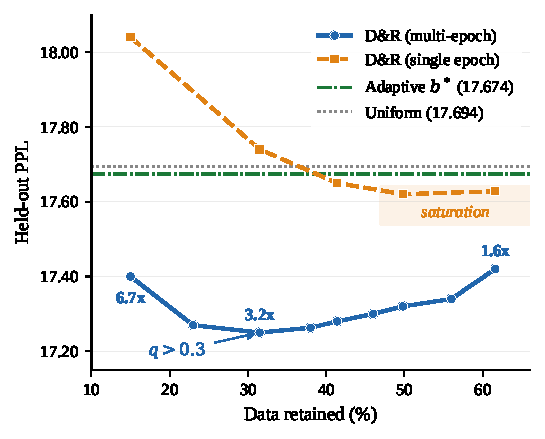
\includegraphics[width=\columnwidth]{dr_dual_curve}
\caption{D\&R threshold--PPL relationship ($\rho{=}0.4$, 3 seeds).
Blue: raw (multi-epoch) PPL with effective epoch counts annotated.
Orange: epoch-matched PPL (single content epoch), saturating at the adaptive $\bstar$ level (green dashed).}
\label{fig:dr_dual_curve}
\end{figure}

\begin{figure}[t]
\centering
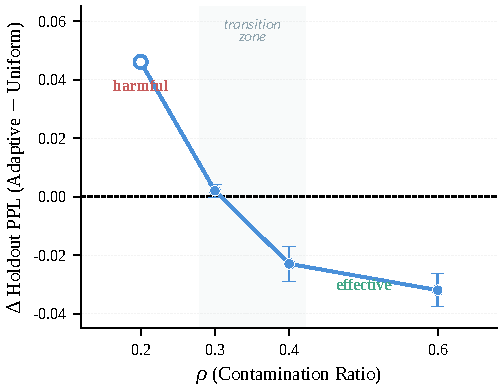
\includegraphics[width=\columnwidth]{delta_vs_rho}
\caption{Effect of contamination ratio on adaptive reweighting effectiveness.
$\Delta$ = adaptive $-$ uniform holdout PPL (lower is better).
Error bars show $\pm$1 SD across seeds.
The method transitions from harmful to beneficial between $\rho{=}0.3$ and $0.4$ (shaded).}
\label{fig:delta_vs_rho}
\end{figure}

\subsection{Robustness and Boundary Conditions}
\label{sec:robustness}

Across three seeds at $\rho = 0.6$, adaptive $\bstar$ ($17.731 \pm 0.004$) directionally outperforms uniform on in-distribution PPL ($17.763 \pm 0.008$, $\Delta{=}{-}0.032$, 3 seeds, paired $t{=}{-}9.95$, $p_{\mathrm{BH}}{=}0.064$), with a larger effect size than at $\rho{=}0.4$ ($\Delta{=}{-}0.023$).
The ablation hierarchy is preserved (Grid 17.634\footnote{Single seed; full per-seed results in Appendix~\ref{app:rho06}.} ${<}$ Adaptive 17.731 ${<}$ Uniform 17.763 ${\approx}$ ESS-only 17.765 ${<}$ Random 17.861), but the ESS-only/uniform gap collapses to effectively zero ($17.763$ vs.\ $17.765$) as ESS binding rises to ${\sim}$49\%.
Random remains substantially worse than uniform (gap 0.098, $\sigma{=}0.027$): detector signal is load-bearing even when the stability constraint dominates; the adaptive method's continued advantage is driven by the $\aeff$ quality constraint, which operates independently of the ESS ceiling.
Three-seed paired comparison confirms $\tau{=}0.7$ outperforms $\tau{=}0.8$ on both holdout and out-of-distribution (OOD) metrics (\S\ref{sec:sensitivity}).

\begin{table}[t]
\centering
\small
\setlength{\tabcolsep}{3pt}
\resizebox{\columnwidth}{!}{%
\begin{tabular}{@{}lccc@{}}
\toprule
\textbf{Method} & \textbf{Epochs} & \textbf{PPL (raw)} $\downarrow$ & \textbf{PPL (ep.-matched)} $\downarrow$ \\
\midrule
D\&R ($q{>}0.3$) & ${\sim}$3.2 & \textbf{17.250} $\pm$ .001 & 17.74 \\
D\&R ($q{>}0.5$) & ${\sim}$2.4 & 17.280 $\pm$ .010 & 17.657 $\pm$ .005 \\
D\&R ($q{>}0.7$) & ${\sim}$2.0 & 17.32 & 17.62 \\
\midrule
Adaptive $\bstar$ & ${\sim}$1.0 & \multicolumn{2}{c}{17.674 $\pm$ .007} \\
Uniform           & ${\sim}$1.0 & \multicolumn{2}{c}{17.697 $\pm$ .008} \\
\bottomrule
\end{tabular}}
\caption{D\&R threshold comparison ($\rho{=}0.4$).
Raw PPL traces a U-shape across thresholds; epoch-matched PPL (single content epoch) decreases monotonically and saturates near the adaptive $\bstar$ level.
D\&R's 0.424 PPL advantage (at $q{>}0.3$) shrinks to $\Delta{=}0.017$ when content epochs are equalized.
All raw PPL values are 3-seed means; epoch-matched values at $q{>}0.3$ and $q{>}0.7$ are single-seed.
Full 9-threshold sweep in Table~\ref{tab:dr_threshold}.}
\label{tab:epoch_match}
\end{table}

\paragraph{Scale.}
At 1.7B parameters (Qwen3-1.7B, $\rho{=}0.4$, $\tau{=}0.8$, 3 seeds), the method scales without degradation but the benefit diminishes.
Adaptive $\bstar$ achieves holdout PPL $13.26$ vs.\ uniform $13.27$ ($\Delta{=}{-}0.013$); OOD results are mixed in direction across domains (OWT $\Delta{=}{-}0.008$, Wiki $\Delta{=}{+}0.013$) and downstream accuracy is unchanged ($\Delta{\approx}{+}0.002$).
The diminished effect is consistent with larger models being more robust to self-generated contamination: Qwen3-1.7B's own outputs are likely closer to its training distribution, reducing the distributional shift that reweighting corrects.
A preliminary Llama-3.2-3B cross-model result (Appendix~\ref{app:cross_model}) shows mixed downstream effects (MMLU $+$1.6 percentage points, HellaSwag $-$0.6 percentage points), leaving cross-architecture generalization as an open question.
\paragraph{Out-of-distribution evaluation.}
To test whether the in-distribution improvement reflects distribution matching, we evaluate all three from-scratch seeds on OpenWebText and Wikipedia.
At $\rho{=}0.4$, adaptive reweighting improves mean PPL on all three evaluation domains: FineWeb $\Delta{=}{-}0.023$ (5 seeds), OpenWebText $\Delta{=}{-}0.026$, Wikipedia $\Delta{=}{-}0.027$ (3 seeds each); downstream accuracy is near-identical (0.5414 vs.\ 0.5415).
OOD improvements exceed the in-distribution gain, indicating genuine quality improvement rather than distribution matching toward the training mixture ($\tau{=}0.8$'s OOD effect is smaller; $\tau{=}0.7$'s advantage reflects active OOD improvement, \S\ref{sec:sensitivity}).

\paragraph{Calibration, not just discrimination.}
Replacing TF-IDF+LR with generative perplexity detectors reverses the advantage across three seeds (GPT-2: AUC\,=\,0.91, ECE\,=\,0.131, $\Delta{=}{+}0.098$; N-gram: AUC\,=\,0.73, ECE\,=\,0.069, $\Delta{=}{+}0.129$; Figure~\ref{fig:overview}b; Appendix~\ref{app:detector}).
The TF-IDF vs.\ GPT-2 contrast (comparable AUC, $2.7{\times}$ ECE gap) isolates calibration as an empirically observed requirement in our self-contamination setting; N-gram's better ECE (0.069) does not compensate for insufficient AUC (0.73), indicating that both discrimination and calibration are jointly necessary (Figure~\ref{fig:overview}b).

\begin{table}[t]
\centering
\small
\setlength{\tabcolsep}{3pt}
\resizebox{\columnwidth}{!}{%
\begin{tabular}{@{}lcccl@{}}
\toprule
\textbf{Method} & \textbf{Seeds} & \textbf{Oracle?} & \textbf{Epochs} & \textbf{Mean PPL} $\downarrow$ \\
\midrule
Grid ($b{=}0.3$) & 3 & post-hoc & 1 & \textbf{17.620} $\pm$ .033 \\
Golden Ratio     & 1 & known $\rho$ & 1 & 17.654 \\
D\&R ($q{>}0.3$) & 3 & post-hoc & ${\sim}$3.2 & \textbf{17.250} $\pm$ .001 \\
\bottomrule
\end{tabular}}
\caption{Auxiliary baselines at $\rho{=}0.4$. Grid-best selected post-hoc from nine candidates (Appendix~\ref{app:grid}). Golden Ratio requires known $\rho$~\citep{he2025golden}. D\&R uses ${\sim}$3.2 content epochs (Table~\ref{tab:epoch_match}).}
\label{tab:aux}
\end{table}

\subsection{Hyperparameter Sensitivity}
\label{sec:sensitivity}

\paragraph{Quality threshold $\tau$.}
$\tau{=}0.7$ outperforms $\tau{=}0.8$ on holdout at both contamination levels ($\rho{=}0.4$: 17.674 vs.\ 17.683; $\rho{=}0.6$: paired $t{=}{-}4.70$, $p{<}0.05$; \S\ref{sec:robustness}) and achieves larger OOD gains ($\rho{=}0.4$: $\Delta{=}{-}0.026$/$-$0.027 vs.\ $-$0.003/$-$0.002; Table~\ref{tab:tau}, Appendix~\ref{app:tau_rho}).
$\tau \in [0.5, 0.8]$ all improve holdout over uniform, while $\tau {>} 0.8$ degrades (Appendix~\ref{app:tau_sweep}).
We also tested per-batch adaptive $\tau$ clamping, which did not improve over fixed thresholds (Appendix~\ref{app:batch_adaptive}).

\paragraph{ESS floor $\nmin$.}
The default $\nmin{=}2$ ($\nmin/B{=}0.5$) is optimal; extremes degrade ($\nmin{=}1$: PPL $17.742{\pm}0.009$, 3 seeds, worse than uniform; $\nmin{=}B$: recovers uniform).
Neither constraint alone improves over uniform ($\nmin{=}1$: $+$0.048; ESS-only: $+$0.043); both must act jointly for the method to outperform uniform training.
The coupling $\nmin{=}\lfloor B/2 \rfloor$ is also empirically motivated: at $B{=}8$, keeping $\nmin{=}2$ (ratio $0.25$) degrades PPL by $+$0.036 vs.\ uniform, whereas $\nmin{=}4$ (ratio $0.5$) yields $\Delta{=}{-}0.052{\pm}0.007$.
Under this coupling, the adaptive advantage monotonically increases across $B \in \{4, 8, 16\}$: $\Delta{=}{-}0.023{\pm}0.006$ (5 seeds), $-$0.052${\pm}$0.007 (3 seeds, $p{=}0.006$), and $-$0.068${\pm}$0.005 (3 seeds), corresponding to $1.0{\times}$, $2.3{\times}$, and $3.0{\times}$ amplification ($p{<}0.01$ at $B \geq 8$).
The gap to grid-best narrows from 0.040 ($B{=}4$) to 0.009 ($B{=}16$, seed\,42; Figure~\ref{fig:batch_amp}).

\begin{figure}[t]
\centering
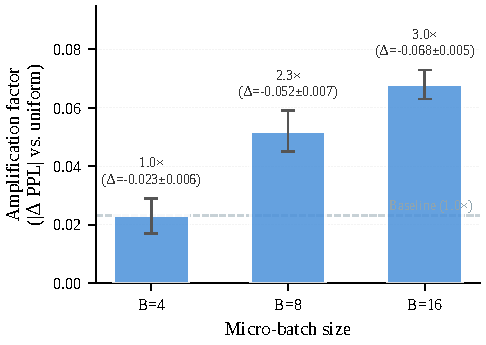
\includegraphics[width=\columnwidth]{batch_size_amplification}
\caption{Batch-size amplification of adaptive reweighting ($\nmin{=}\lfloor B/2 \rfloor$).
The adaptive advantage over uniform increases monotonically with micro-batch size, from $1.0{\times}$ ($B{=}4$) to $3.0{\times}$ ($B{=}16$); $\Delta$ values and $\pm$1\,SD shown above each bar.}
\label{fig:batch_amp}
\end{figure}

\paragraph{Constraint regime.}
\label{sec:regime}
Over 24{,}412 micro-batches (seed\,42), 5.8\% are clean ($\aeff(0) \geq \tau$, $\bstar{=}0$), ${\sim}$50\% are $\aeff$-binding (quality constraint dominates), and ${\sim}$44\% are ESS-binding (stability constraint dominates); the distribution is stable across seeds (coefficient of variation ${<}2\%$; Figure~\ref{fig:regime_decomp}).
The $\aeff$-binding majority indicates that detector quality signal, not training stability, is the primary bottleneck, reinforcing the calibration requirement (\S\ref{sec:robustness}).

\begin{figure}[t]
\centering
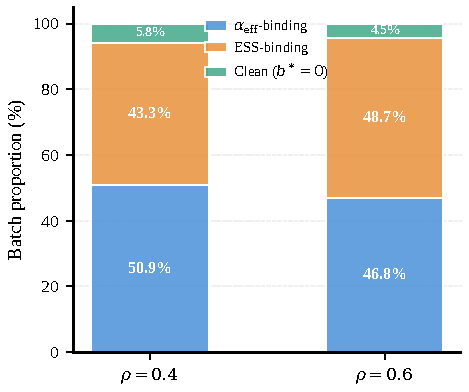
\includegraphics[width=\columnwidth]{constraint_regime_decomposition}
\caption{Constraint regime decomposition at two contamination levels (seed\,42).
At $\rho{=}0.4$, ${\sim}$50\% of batches are $\aeff$-binding and ${\sim}$44\% ESS-binding, with ${\sim}$6\% clean; at $\rho{=}0.6$, the constraints are nearly balanced (${\sim}$49\% ESS-binding, ${\sim}$47\% $\aeff$-binding).}
\label{fig:regime_decomp}
\end{figure}


\section{Discussion}
\label{sec:discussion}
\paragraph{D\&R as the strongest strategy.}
D\&R outperforms all reweighting methods by $0.35$--$0.42$ PPL (Table~\ref{tab:epoch_match}), but epoch-matched controls attribute ${>}$95\% of this advantage to multi-epoch exposure on filtered data rather than superior per-token learning.
This benefit was invisible in \citet{drayson2025detection}, where from-scratch pretraining rarely completes one epoch; in continued pretraining, it becomes the dominant factor.

\paragraph{When uniform beats reweighting.}
Table~\ref{tab:decision} summarizes three prerequisites for effective soft reweighting: (i)~sufficient detector discrimination \emph{and} calibration (AUC\,$\geq$\,0.9, ECE\,$\leq$\,0.05; \S\ref{sec:robustness}); (ii)~contamination $\rho \geq 0.4$, below which the method degrades ($+$0.046 at $\rho{=}0.2$; Appendix~\ref{app:rho02}) with a sharp transition in $[0.3, 0.4]$ (Figure~\ref{fig:delta_vs_rho}, Appendix~\ref{app:rho03}); (iii)~generator--trainee mismatch (at 1.7B the benefit diminishes to $\Delta{=}{-}0.013$ with OOD mixed).
When any condition is violated, uniform is the safer default.

\begin{table}[t]
\centering
\small
\setlength{\tabcolsep}{3pt}
\resizebox{\columnwidth}{!}{%
\begin{tabular}{@{}lcll@{}}
\toprule
\textbf{Condition} & \textbf{Observed?} & \textbf{Evidence} & \textbf{$\Delta$ PPL} \\
\midrule
Detector AUC $\geq 0.9$ & Yes & N-gram (0.73) degrades & $+$0.129 \\
Detector ECE $\leq 0.05$ & Yes & GPT-2 (0.131) degrades & $+$0.098 \\
Contamination $\rho \geq 0.4$ & Yes & $\rho{=}0.2$ degrades & $+$0.046 \\
Generator $\neq$ trainee & Tentative & 1.7B: $\Delta{=}{-}0.013$, OOD mixed & -- \\
\bottomrule
\end{tabular}}
\caption{Decision summary for practitioners.
$\Delta$ values are relative to uniform (positive = worse).
When any observed condition is violated, uniform is the safer default.}
\label{tab:decision}
\end{table}

\paragraph{Effect size and downstream impact.}
The in-distribution improvement ($\Delta{=}{-}0.023$ at $\rho{=}0.4$) does not transfer to downstream accuracy (0.5414 vs.\ 0.5415, 3 seeds; Appendix~\ref{app:downstream}), consistent with nonlinear PPL-to-accuracy transfer~\citep{tay2022scale,ye2025mixing}; the paradigm's impact at current scales is modest (Appendix~\ref{app:power}; Table~\ref{tab:appendix_summary}).

\paragraph{Limitations of $\aeff$ as a proxy.}
The $\aeff$ diagnostic correlates with the true batch-level real fraction at Pearson $r \approx 0.79$ (${\sim}$63\% of variance; Appendix~\ref{app:alpha_validation}), stable across seeds (Spearman $\rho_s \geq 0.86$; Table~\ref{tab:alpha_corr_perseed}).
The ceiling is set by detector calibration, not batch size.
Because \citet{wang2026survive}'s convergence guarantee requires the \emph{true} real fraction, the ${\sim}$37\% unexplained variance means some batches satisfying $\aeff \geq \tau$ may have true fractions below $\tau$; the $\nmin$ constraint mitigates this by capping $b$ at the ESS floor~\citep{owen2013mc}.


\section{Conclusion}
\label{sec:conclusion}
We identify three effectiveness conditions for detect-and-reweight: (i)~D\&R is the strongest method in our setting, with multi-epoch exposure on filtered data accounting for ${>}$95\% of its advantage over reweighting; (ii)~detector calibration alongside discrimination, as high-AUC detectors with poor calibration degrade PPL below uniform; and (iii)~minimum intervention over unconstrained maximization, supported by the ESS-only ablation and the fixed-$b$ grid curve (Figure~\ref{fig:grid_b_trend}).
A dual-constrained adaptive $\bstar$ implementing these principles improves over uniform training at $\rho \geq 0.4$ without per-model tuning (Table~\ref{tab:decision}), though without measurable downstream gains at 0.6B scale.
Whether these conditions hold at full pretraining scale ($>$100B tokens), where contamination ratios are lower but corpora are harder to curate, is the central open question; a second priority is extending the detector--calibration axis to neural classifiers whose ECE profiles differ qualitatively from the TF-IDF family tested here.


\section*{Limitations}
\label{sec:limitations}
\begin{itemize}[nosep,leftmargin=*]
\item \textbf{Scope.}
All experiments use Qwen3 (0.6B and 1.7B) under self-contamination with 132--200M tokens of continued pretraining.
Generalization to other architectures, full pretraining scale ($>$100B tokens), or realistic multi-source web contamination, where generator-corpus distribution mismatch may reduce detector accuracy, remains untested.

\item \textbf{Detector coverage.}
Only three detectors from two families (discriminative TF-IDF+LR and generative perplexity scorers) were evaluated; fine-tuned neural classifiers (e.g., ModernBERT) and zero-shot methods (e.g., DetectGPT, Binoculars) remain untested, so the AUC/ECE thresholds reported here may shift with broader detector coverage.

\item \textbf{Evaluation scope.}
Our primary metric is held-out perplexity; downstream accuracy is unchanged across conditions (Appendix~\ref{app:downstream}), so the practical benefit at 0.6B scale is limited to distributional quality rather than task performance.
\end{itemize}


\bibliography{references}

\appendix
\section{Proofs}
\label{app:proofs}

\begin{proposition}[$\alpha_{\mathrm{eff}}$ monotonicity]
\label{prop:monotone}
$\alpha_{\mathrm{eff}}(b)$ is non-decreasing in $b$, and strictly increasing whenever the batch contains at least two samples with distinct $q$-values.
\end{proposition}

\begin{proof}[Proof of Proposition~\ref{prop:monotone}]
Let $w_i(b) = (1 - q_i)^b$, $W(b) = \sum_{j=1}^B w_j(b)$, and $\pi_i(b) = w_i(b) / W(b)$.
Then
\begin{equation*}
  \alpha_{\mathrm{eff}}(b) = \sum_{i=1}^{B} \pi_i(b)\, (1 - q_i).
\end{equation*}
Taking the derivative with respect to $b$:
\begin{align*}
  \frac{d\pi_i}{db}
  &= \pi_i \!\left(\frac{d \ln w_i}{db} - \frac{d \ln W}{db}\right) \\
  &= \pi_i \!\left(\ln(1{-}q_i) - \textstyle\sum_j \pi_j \ln(1{-}q_j)\right).
\end{align*}
Substituting,
\begin{align*}
  \frac{d\alpha_{\mathrm{eff}}}{db}
  &= \sum_i (1{-}q_i)\, \pi_i \!\left(\ln(1{-}q_i) - \mathbb{E}_{\pi}[\ln(1{-}q)]\right) \\
  &= \mathrm{Cov}_{\pi}\!\bigl(1{-}q_i,\, \ln(1{-}q_i)\bigr).
\end{align*}
Since $(1{-}q_i)$ and $\ln(1{-}q_i)$ are both increasing functions of $(1{-}q_i)$, they are positively associated, so the covariance is non-negative.
\end{proof}

\begin{proposition}[ESS monotonicity]
\label{prop:ess_mono}
$\mathrm{ESS}(b)$ is non-increasing in $b$, and strictly decreasing whenever the batch contains at least two samples with distinct $q$-values.
\end{proposition}

\begin{proof}
Write $\mathrm{ESS}(b) = 1 / \sum_i \pi_i(b)^2$, where $\pi_i(b) = w_i(b) / W(b)$.
The denominator $\sum_i \pi_i^2$ is the Herfindahl index $H$.
Differentiating $H$ with respect to $b$:
\begin{equation*}
  \frac{dH}{db} = 2 \sum_i \pi_i^2 \bigl(\ln(1{-}q_i) - \mathbb{E}_{\pi}[\ln(1{-}q)]\bigr).
\end{equation*}
Since $\pi_i \propto (1{-}q_i)^b$, larger $\pi_i$ implies larger $\ln(1{-}q_i)$; the $\pi^2$-weighted sum assigns greater mass to terms where $\ln(1{-}q_i) > \mathbb{E}_\pi[\ln(1{-}q)]$, so $dH/db \geq 0$, with strict inequality when at least two $q$-values differ.
Thus $H$ is non-decreasing and $\mathrm{ESS} = 1/H$ is non-increasing.
This is a standard property of exponential tilting~\citep{kish1965survey,owen2013mc}.
\end{proof}

\section{Algorithm Details}
\label{app:algorithm}

\begin{algorithm}[h]
\caption{Per-batch adaptive $b^{*}$ selection}
\label{alg:bstar}
\begin{algorithmic}[1]
\REQUIRE Batch scores $\{q_i\}_{i=1}^{B}$, threshold~$\tau$, ESS floor~$n_{\min}$, bound~$b_{\max}$, tol.~$\varepsilon$
\ENSURE Optimal sharpening exponent $b^{*}$
\IF{$\alpha_{\mathrm{eff}}(0) \geq \tau$}
  \STATE \textbf{return} $0$ \COMMENT{clean batch}
\ENDIF
\STATE $b_\tau \gets \textsc{Bisect}(\alpha_{\mathrm{eff}}(\cdot){=}\tau,\; [0, b_{\max}],\; \varepsilon)$
\IF{$\mathrm{ESS}(b_\tau) \geq n_{\min}$}
  \STATE \textbf{return} $b_\tau$ \COMMENT{$\alpha_{\mathrm{eff}}$-binding}
\ELSE
  \STATE $b_{\mathrm{ESS}} \gets \textsc{Bisect}(\mathrm{ESS}(\cdot){=}n_{\min},\; [0, b_{\max}],\; \varepsilon)$
  \STATE \textbf{return} $b_{\mathrm{ESS}}$ \COMMENT{ESS-binding}
\ENDIF
\end{algorithmic}
\end{algorithm}

\begin{figure}[h]
\centering
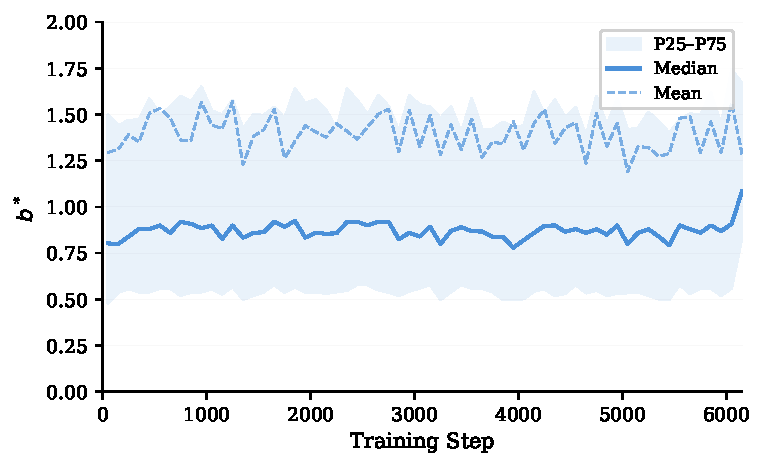
\includegraphics[width=\columnwidth]{bstar_trajectory_adaptive_fix}
\caption{Adaptive $\bstar$ trajectory over 6{,}103 training steps (seed\,42, $\rho{=}0.4$).
The exponent alternates between clean ($\bstar{=}0$), $\aeff$-binding, and ESS-binding regimes with no systematic drift, reflecting per-batch adaptation to local $q$-score composition.}
\label{fig:bstar_traj}
\end{figure}
We compute $\bstar$ at the micro-batch level ($B{=}4$) rather than the effective batch ($B{=}16$ after gradient accumulation) because $q$-score statistics exhibit sufficient variance within micro-batches: Spearman $r{=}0.699$ with the true real fraction, and at $B{=}16$ the adaptive advantage amplifies $3.0{\times}$ ($\Delta{=}{-}0.068{\pm}0.005$; \S\ref{sec:sensitivity}).

\section{Grid Search Details}
\label{app:grid}

Table~\ref{tab:grid_full} reports held-out PPL for all grid-$b$ values at $\rho = 0.4$ (seed\,42).

\begin{table}[h]
\centering
\small
\begin{tabular}{@{}cc@{}}
\toprule
$b$ & PPL $\downarrow$ \\
\midrule
0.1 & 17.657 \\
0.2 & 17.640 \\
0.3 & \textbf{17.640} \\
0.5 & 17.651 \\
1.0 & 17.692 \\
1.5 & 17.718 \\
2.0 & 17.741 \\
3.0 & 17.774 \\
5.0 & 17.818 \\
\bottomrule
\end{tabular}
\caption{Full grid search results ($\rho{=}0.4$, seed\,42).
$b \in [0.1, 0.5]$ forms a broad plateau (three-seed mean for $b{=}0.1$: $17.655 \pm 0.009$); $b{=}0.3$ is the post-hoc best.}
\label{tab:grid_full}
\end{table}

\section{Quality Threshold Sweep}
\label{app:tau_sweep}

\begin{table}[h]
\centering
\small
\resizebox{\columnwidth}{!}{%
\begin{tabular}{@{}ccccccc@{}}
\toprule
$\tau$ & Holdout $\downarrow$ & $\Delta_{\text{H}}$ & OWT $\downarrow$ & $\Delta_{\text{O}}$ & Wiki $\downarrow$ & $\Delta_{\text{W}}$ \\
\midrule
0.50 & 17.688 & $-$0.006 & -- & -- & -- & -- \\
0.60 & 17.681 & $-$0.013 & -- & -- & -- & -- \\
0.70$^\star$ & \textbf{17.674{\tiny$\pm$.006}} & $\boldsymbol{-}$\textbf{0.020} & \textbf{18.347{\tiny$\pm$.003}} & $\boldsymbol{-}$\textbf{0.028} & \textbf{15.330{\tiny$\pm$.015}} & $\boldsymbol{-}$\textbf{0.029} \\
0.80$^\star$ & 17.683{\tiny$\pm$.006} & $-$0.011 & 18.370{\tiny$\pm$.005} & $-$0.005 & 15.350 & $-$0.009 \\
0.90 & 17.712 & $+$0.018 & -- & -- & -- & -- \\
0.95 & 17.723 & $+$0.029 & -- & -- & -- & -- \\
\bottomrule
\end{tabular}}
\caption{Quality threshold sweep ($\nmin{=}2$, $\rho{=}0.4$).
$\Delta$ relative to 3-seed uniform baseline (Holdout 17.694, OWT 18.375, Wiki 15.359).
$^\star$\,$\tau{=}0.7$: 5-seed mean (SD from 5 seeds); $\tau{=}0.8$: 3 from-scratch seeds (Appendix~\ref{app:resume_artifact}). The 5-seed comparison in Table~\ref{tab:main} yields $\Delta{=}{-}0.023$.
Other values from single-seed exploratory sweep (seed\,42, holdout only).
$\tau{=}0.7$ achieves the lowest holdout and largest OOD gains ($|\Delta| \geq 0.028$); $\tau{=}0.8$'s OOD effect is smaller ($|\Delta| \leq 0.009$).}
\label{tab:tau}
\end{table}

\section{Batch-Adaptive $\tau$}
\label{app:batch_adaptive}

We tested a per-batch adaptive variant that clamps $\tau$ between 0.5 and the fixed threshold based on local $\aeff(0)$, allowing the quality floor to relax in batches with low estimated real fraction.
At both contamination levels ($\rho \in \{0.4, 0.6\}$), the adaptive variant did not outperform the fixed threshold (single-seed exploratory at each level), suggesting the quality constraint does not require adaptation to local contamination density.
This supports the ``two hyperparameters with good defaults'' characterization: neither $\tau$ nor $\nmin$ benefits from per-batch tuning.

\section{\texorpdfstring{$\tau$--$\rho$}{tau-rho} Rank Preservation}
\label{app:tau_rho}

Figure~\ref{fig:tau_rho_rank} shows the $\tau$--PPL relationship at two contamination levels.

\begin{figure}[h]
\centering
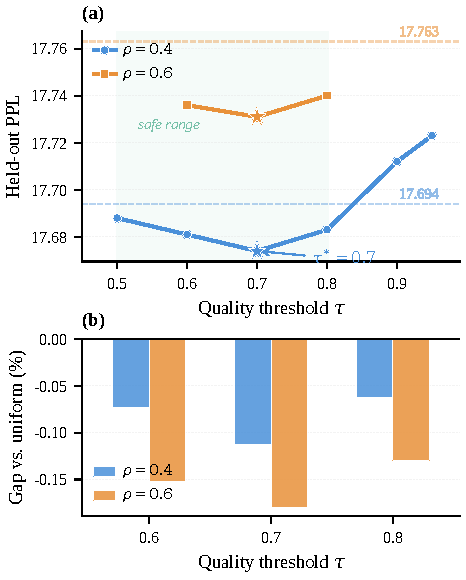
\includegraphics[width=\columnwidth]{tau_rho_rank_preservation}
\caption{(a) Held-out PPL as a function of quality threshold $\tau$ at $\rho \in \{0.4, 0.6\}$.
$\tau{=}0.7$ and $\tau{=}0.8$ yield comparable holdout PPL at $\rho{=}0.4$; at $\rho{=}0.6$, $\tau{=}0.7$ is statistically better (paired $t{=}{-}4.70$, $p{<}0.05$, 3 seeds, $\Delta{=}{-}0.005$). $\tau{=}0.7$ also achieves lower OOD perplexity at both levels ($\rho{=}0.6$: $\Delta_{\text{OWT}}{=}{-}0.014$, $\Delta_{\text{Wiki}}{=}{-}0.013$, 2 seeds).
(b) Normalized PPL gap relative to uniform at shared $\tau$ values.}
\label{fig:tau_rho_rank}
\end{figure}

\section{Hybrid and Threshold Comparison}
\label{app:hybrid}

Table~\ref{tab:hybrid} compares method families across contamination levels.
Table~\ref{tab:dr_threshold} shows D\&R sensitivity to the detection threshold at both full training length and epoch-matched settings.
Raw PPL traces a U-shaped curve with a minimum at $q{>}0.3$ (17.250, 3 seeds), but this curve conflates filtering quality with multi-epoch exposure: aggressive thresholds retain less data and repeat it more often.
Epoch-matched comparisons (rightmost column of Table~\ref{tab:dr_threshold}) remove the multi-epoch confound: the U-shape vanishes and PPL decreases monotonically, saturating near the adaptive $\bstar$ level at $q{\geq}0.5$.
Figure~\ref{fig:dr_dual_curve} visualizes the two curves.

\begin{table}[h]
\centering
\small
\begin{tabular}{@{}lcc@{}}
\toprule
\textbf{Method} & $\rho{=}0.4$ & $\rho{=}0.6$ \\
\midrule
Uniform & 17.694 & 17.766 \\
Adaptive $\bstar$ & 17.689 & 17.740 \\
Hybrid ($q{>}0.95$ + adaptive) & 17.514 & 17.530$^*$ \\
Detect \& Remove ($q{>}0.5$) & 17.285 & -- \\
Detect \& Remove ($q{>}0.3$) & 17.250 & -- \\
\bottomrule
\end{tabular}
\caption{Method comparison across contamination levels (seed\,42, $\tau{=}0.8$).
$^*$Hybrid at $\rho{=}0.6$ filters high-confidence synthetic ($q{>}0.95$), reducing effective $\rho$ to ${\approx}0.4$; PPL is not directly comparable to $\rho{=}0.6$ baselines.}
\label{tab:hybrid}
\end{table}

\begin{table}[h]
\centering
\small
\setlength{\tabcolsep}{3pt}
\begin{tabular}{@{}ccccc@{}}
\toprule
\textbf{Thresh.} & \textbf{Ret.\ \%} & \textbf{Epochs} & \textbf{Raw PPL} $\downarrow$ & \textbf{Ep.-matched} $\downarrow$ \\
\midrule
$q > 0.1$ & 15.0\% & ${\sim}$10.0 & 17.40 & 18.04 \\
$q > 0.2$ & ${\sim}$23\% & ${\sim}$5.0 & 17.27 & -- \\
$q > 0.3$ & 31.5\% & ${\sim}$3.2 & \textbf{17.250}$^\dagger$ & 17.74 \\
$q > 0.4$ & ${\sim}$38\% & ${\sim}$2.8 & 17.26 & -- \\
$q > 0.5$ & 41.4\% & ${\sim}$2.4 & 17.28 & 17.65 \\
$q > 0.6$ & ${\sim}$46\% & ${\sim}$1.7 & 17.30 & -- \\
$q > 0.7$ & 49.8\% & ${\sim}$2.0 & 17.32 & 17.62 \\
$q > 0.8$ & ${\sim}$56\% & ${\sim}$1.3 & 17.34 & -- \\
$q > 0.9$ & 61.6\% & ${\sim}$1.1 & 17.42 & 17.628 \\
\bottomrule
\end{tabular}
\caption{D\&R threshold sensitivity ($\rho{=}0.4$, seed\,42 unless noted).
Raw PPL traces a U-shaped curve (minimum at $q{>}0.3$); epoch-matched PPL (single content epoch) decreases monotonically and saturates near the adaptive $\bstar$ level (${\approx}$17.65) at $q{\geq}0.5$; the U-shape is thus a multi-epoch artifact.
$^\dagger$\,3-seed mean $17.250 \pm 0.001$.}
\label{tab:dr_threshold}
\end{table}

See Figure~\ref{fig:dr_dual_curve} (\S\ref{sec:main-results}) for the dual-curve visualization.

\section{Downstream Task Evaluation}
\label{app:downstream}

Table~\ref{tab:downstream} reports downstream benchmark accuracy for adaptive vs.\ uniform training at $\rho{=}0.4$ (seed\,42, Qwen3-0.6B).
Across multiple seeds, downstream differences are mixed in direction and uniformly within standard error, indicating that adaptive reweighting has no meaningful downstream impact.

\begin{table}[h]
\centering
\small
\resizebox{\columnwidth}{!}{%
\begin{tabular}{@{}llccc@{}}
\toprule
\textbf{Benchmark} & \textbf{Metric} & \textbf{Adaptive} & \textbf{Uniform} & $\boldsymbol{\Delta}$ \\
\midrule
\multicolumn{5}{@{}l}{\textit{Seed 42 (checkpoint resume)}} \\
ARC-Challenge & acc\_norm & 0.343 & 0.348 & $-$0.005 \\
ARC-Easy & acc & 0.650 & 0.657 & $-$0.007 \\
HellaSwag & acc\_norm & 0.479 & 0.484 & $-$0.005 \\
PIQA & acc & 0.687 & 0.686 & $+$0.001 \\
WinoGrande & acc & 0.578 & 0.586 & $-$0.008 \\
\midrule
\multicolumn{5}{@{}l}{\textit{From-scratch 2-seed mean (seeds 123, 456)}} \\
\multicolumn{3}{@{}l}{Mean $\Delta$ across 5 tasks} & & $+$0.001 \\
\multicolumn{3}{@{}l}{Direction} & \multicolumn{2}{c}{mixed (seed 123: 3/5$-$; seed 456: 3/5$+$)} \\
\bottomrule
\end{tabular}}
\caption{Downstream benchmarks (Qwen3-0.6B, $\rho{=}0.4$).
Seed\,42 used a checkpoint-resumed adaptive model; from-scratch seeds (123, 456) show mixed direction with mean $|\Delta| \leq 0.01$.
All differences within standard error ($\pm 0.01$).
Models use $\tau{=}0.8$; $\tau{=}0.7$ yields identical 3-seed means (0.5414).}
\label{tab:downstream}
\end{table}

\section{Higher Contamination Details}
\label{app:rho06}

Table~\ref{tab:rho06} reports results at $\rho{=}0.6$.
The full five-method ablation preserves the hierarchy from $\rho{=}0.4$ across all three seeds: Grid ${<}$ Adaptive ${<}$ Uniform ${\approx}$ ESS-only ${<}$ Random.

\begin{table}[h]
\centering
\small
\resizebox{\columnwidth}{!}{%
\begin{tabular}{@{}lcccc@{}}
\toprule
\textbf{Method} & \textbf{Seed 42} & \textbf{Seed 123} & \textbf{Seed 456} & \textbf{Mean} \\
\midrule
Grid ($b{=}0.3$)$^\ddagger$ & \textbf{17.634} & -- & -- & -- \\
Adaptive $\bstar$ & 17.735 & 17.727 & 17.732 & 17.731 $\pm$ .004 \\
Uniform           & 17.766 & 17.754 & 17.770 & 17.763 $\pm$ .008 \\
ESS-only          & 17.770 & 17.760 & 17.760 & 17.763 $\pm$ .006 \\
Random $\mathcal{U}(0,2)$ & 17.832 & 17.870 & 17.880 & 17.861 $\pm$ .025 \\
\bottomrule
\end{tabular}}
\caption{Results at $\rho{=}0.6$ (Qwen3-0.6B, $\nmin{=}2$).
Adaptive uses $\tau{=}0.7$ (consistent with main results); other methods are $\tau$-independent.
$^\ddagger$Post-hoc oracle; seed\,42 only.
Adaptive vs.\ Uniform: $\Delta{=}{-}0.032$, paired $t{=}{-}15.4$, $p{=}0.004$ (full precision; 3dp rounding yields $t{=}{-}9.95$, $p{=}0.010$).
ESS-only collapses onto Uniform (both $17.763$); Random ($17.861$) confirms detector signal is load-bearing.}
\label{tab:rho06}
\end{table}

The ESS-only/Uniform gap collapses from 0.043 at $\rho{=}0.4$ to 0.000 at $\rho{=}0.6$ (three-seed means: both $17.763$); ESS binding rises to ${\sim}$49\% of batches (from ${\sim}$43\% at $\rho{=}0.4$), and the constraints become nearly balanced rather than $\aeff$-dominant.
The adaptive method maintains its advantage ($\Delta{=}{-}0.032$, consistent across seeds) through the $\aeff$ quality constraint, which operates independently of the ESS ceiling.
Random reweighting ($17.861 \pm 0.025$) is substantially worse than Uniform, with the highest cross-seed variance; uninformed weights add noise without corrective signal.
The Adaptive-vs-Grid gap is 0.054 at $\rho{=}0.4$ (mean-to-mean, consistent with Table~\ref{tab:aux}) and 0.097 at $\rho{=}0.6$ (adaptive 3-seed mean vs.\ grid seed\,42; the $\rho{=}0.6$ grid result is preliminary and may not generalize across seeds).

\section{\texorpdfstring{$\alpha_{\mathrm{eff}}$}{alpha-eff} Proxy Validation}
\label{app:alpha_validation}

Table~\ref{tab:alpha_corr} reports the correlation between $\aeff(0)$ (the detector-based proxy at $b{=}0$) and the true batch-level real fraction $\alpha_{\mathrm{true}}$, computed over all training batches at $\rho{=}0.4$ (seed\,42).

\begin{table}[h]
\centering
\small
\begin{tabular}{@{}ccccc@{}}
\toprule
$B$ & Pearson $r$ & Spearman $r$ & MAE$\downarrow$ & Bias \\
\midrule
4  & 0.706 & 0.699 & 0.114 & $-$0.029 \\
8  & 0.697 & 0.683 & 0.097 & $-$0.027 \\
16 & 0.707 & 0.691 & 0.075 & $-$0.031 \\
\bottomrule
\end{tabular}
\caption{Correlation between $\aeff(0)$ and true batch-level real fraction across batch sizes ($\rho{=}0.4$, seed\,42).
Values use a binarized proxy $\hat{r}_i = \mathbf{1}[q_i \leq 0.5]$ for discrete comparison; the continuous formulation used during training (\S\ref{sec:method}) achieves $r \approx 0.77$--$0.79$ depending on batch size.
The consistent negative bias (${\approx}{-}0.03$) indicates that $\aeff$ slightly underestimates the true real fraction, biasing the method toward conservative intervention.}
\label{tab:alpha_corr}
\end{table}

Mean absolute error (MAE) decreases with batch size (0.114 $\to$ 0.075) as expected from averaging, but the rank-order information that drives $\bstar$ selection is already well-captured at $B{=}4$.

\paragraph{Cross-seed stability.}
Table~\ref{tab:alpha_corr_perseed} reports the correlation between $\aeff$ and the batch mean $q$-score ($\bar{q}$, computed from known labels) across all three seeds.

\begin{table}[h]
\centering
\small
\begin{tabular}{@{}cccc@{}}
\toprule
\textbf{Seed} & Pearson $r(\aeff, \bar{q})$ & Spearman $\rho_s$ & $\bstar{=}0$ (\%) \\
\midrule
42  & 0.8019 & 0.8761 & 5.8 \\
123 & 0.7994 & 0.8692 & 5.7 \\
456 & 0.8006 & 0.8749 & 5.9 \\
\midrule
\textbf{Spread} & 0.0025 & 0.0069 & 0.2 \\
\bottomrule
\end{tabular}
\caption{Per-seed $\aeff$--$\bar{q}$ correlation ($\rho{=}0.4$, $B{=}4$).
Cross-seed spread is $<$0.003 for Pearson $r$ and $<$0.007 for Spearman $\rho_s$, indicating stable proxy fidelity across random seeds.
$r(\aeff, \bar{q}) = 0.80$ measures the proxy's fidelity to batch composition; the ground-truth correlation $r(\aeff, \text{true real fraction}) \approx 0.79$ (\S\ref{sec:discussion}) is slightly lower due to detector noise.
The per-seed table demonstrates cross-seed stability rather than superseding the ground-truth estimate.}
\label{tab:alpha_corr_perseed}
\end{table}

\section{Detector Comparison}
\label{app:detector}

See Figure~\ref{fig:overview}b (\S\ref{sec:robustness}) for the detector requirements visualization.

Table~\ref{tab:detector} compares three detector families for adaptive reweighting.
The discriminative TF-IDF+LR detector (ECE\,=\,0.048) produces the only improvement over uniform.
The TF-IDF vs.\ GPT-2 contrast (comparable AUC: 0.94 vs.\ 0.91, but $2.7{\times}$ ECE gap: 0.048 vs.\ 0.131) isolates calibration as an empirically observed requirement; however, N-gram's better ECE (0.069) does not compensate for its low AUC (0.73); both sufficient discrimination and good calibration are jointly necessary in our setting.
TF-IDF+LR's $q$-scores have reliable probabilistic semantics, so the $\aeff$ proxy accurately tracks batch quality.
Generative detectors assign high $q$-scores to fluent, predictable human text (false positives concentrated among high-quality samples), systematically inflating $\aeff$ for clean batches and deflating it for contaminated ones, which inverts the minimum-intervention logic.

\begin{table}[h]
\centering
\small
\resizebox{\columnwidth}{!}{%
\begin{tabular}{@{}llccccc@{}}
\toprule
\textbf{Detector} & \textbf{Type} & \textbf{AUC} & \textbf{ECE} & \textbf{Mean PPL} & $\boldsymbol{\Delta}$ \\
\midrule
TF-IDF+LR & Discriminative & 0.94 & 0.048 & 17.650{\tiny$\pm$.010} & $-$0.044 \\
GPT-2 PPL & Generative & 0.91 & 0.131 & 17.792{\tiny$\pm$.005} & $+$0.098 \\
N-gram PPL & Generative & 0.73 & 0.069 & 17.823{\tiny$\pm$.003} & $+$0.129 \\
\bottomrule
\end{tabular}}
\caption{Detector comparison for adaptive reweighting ($\rho{=}0.4$, $\tau{=}0.8$, 3 seeds).
Uniform baseline PPL\,=\,17.694.
$\Delta$ = Adaptive $-$ Uniform (negative is better).
TF-IDF+LR calibrated via temperature scaling.
The $\tau$ confound is conservative: TF-IDF+LR at $\tau{=}0.7$ achieves 17.674 (Table~\ref{tab:main}).}
\label{tab:detector}
\end{table}

\section{Detector and Synthetic Data Details}
\label{app:detector_details}

\paragraph{TF-IDF+LR detector.}
TF-IDF features (unigrams + bigrams, max 50{,}000 features, sublinear TF) fed to Logistic Regression (C\,=\,1.0, L2 penalty, solver\,=\,lbfgs, max\_iter\,=\,100).
Trained on a held-out labeled split (10K documents per class).
Post-hoc temperature scaling applied when uncalibrated ECE exceeds 0.05: a scalar $T$ is searched via \texttt{scipy.optimize.minimize\_scalar} over $[0.1, 10.0]$ on a 20\% stratified validation split, yielding $T{=}0.204$ (ECE reduced from 0.12 to 0.048).
The detector is selected automatically from six configurations as the first satisfying AUC $\in [0.85, 0.98]$ and mid-range score ratio $\geq 5\%$.

\paragraph{Synthetic data generation.}
Continuations generated with Qwen3-0.6B (self-generation) using nucleus sampling ($p{=}0.95$, $T{=}0.8$), producing up to 384 tokens per continuation from a 128-token prefix prompt (512 total), targeting ${\sim}$100M synthetic tokens.
Source prompts are the first 128 tokens of randomly sampled FineWeb documents, used as prefix continuations.
Injected at token-level ratio $\rho$ via uniform random mixing across the training corpus.

\section{Low Contamination Analysis}
\label{app:rho02}

At $\rho{=}0.2$, the adaptive method degrades by $+$0.046 PPL relative to uniform (0.26\% relative, seed\,42).
The detector's mean $q$-score at this contamination level is 0.393 (vs.\ 0.487 at $\rho{=}0.4$), indicating that many clean samples receive moderate $q$-scores, blurring the provenance signal.
The regime decomposition reveals 13.7\% clean batches ($\bstar{=}0$), 60.1\% $\aeff$-binding, and 26.3\% ESS-binding, with mean $\bstar{=}1.735$ in reweighted batches.
The high $\aeff$-binding rate (60.1\% vs.\ ${\sim}$50\% at $\rho{=}0.4$) means the method actively intervenes rather than defaulting to $\bstar{=}0$, but the unreliable signal causes it to suppress useful training data.
This is consistent with the generative detector failures: when $q$-scores do not reliably separate provenance, the minimum intervention framework amplifies the error rather than correcting it.
The effective range of the method is $\rho \geq 0.4$ with $\tau \in [0.7, 0.8]$ (\S\ref{sec:sensitivity}); lower $\tau$ values may extend the range but have not been tested at $\rho{=}0.2$.

\section{Cross-Model Transfer}
\label{app:cross_model}

Table~\ref{tab:cross_model} reports a single exploratory run with Llama-3.2-3B as a cross-generator (synthetic data generated by Llama, training on Qwen3-0.6B); this does not establish generality.
Results are mixed: MMLU improves while HellaSwag slightly degrades, consistent with the pattern observed in Qwen3-1.7B downstream evaluation (\S\ref{sec:robustness}).
Perplexity comparison omitted due to inconsistent evaluation configurations; checkpoints were not retained for re-evaluation.

\begin{table}[h]
\centering
\small
\resizebox{\columnwidth}{!}{%
\begin{tabular}{@{}lccc@{}}
\toprule
\textbf{Metric} & \textbf{Uniform} & \textbf{Adaptive} & $\boldsymbol{\Delta}$ \\
\midrule
MMLU (5-shot) & 51.85\% $\pm$ .41 & 53.42\% $\pm$ .41 & $+$1.57pp \\
HellaSwag (10-shot, acc\_norm) & 73.08\% $\pm$ .44 & 72.49\% $\pm$ .45 & $-$0.59pp \\
\bottomrule
\end{tabular}}
\caption{Cross-model transfer: Llama-3.2-3B generator, Qwen3-0.6B trainer ($\rho{=}0.4$, single seed).
Mixed results reflect evaluation-set distribution sensitivity rather than consistent quality differences.}
\label{tab:cross_model}
\end{table}

\section{Checkpoint Resume Artifact}
\label{app:resume_artifact}

The checkpoint-resume artifact described here affected early $\tau{=}0.8$ experiments only.
All results in Tables~\ref{tab:main}--\ref{tab:epoch_match} use independent from-scratch training ($\tau{=}0.7$; Table~\ref{tab:main} Adaptive/Uniform: five seeds, others: three seeds).

The adaptive model for seed\,42 in early $\tau{=}0.8$ runs was trained with a checkpoint-resumed run whose first ${\sim}$1{,}000 steps used different hyperparameters (learning rate warmup, gradient accumulation configuration) than seeds 123 and 456, which were trained from scratch.
The resume artifact inflates the in-distribution effect ($\Delta{=}{-}0.041$ resume vs.\ $\Delta{=}{-}0.005$ from-scratch at $\tau{=}0.8$) and reverses the out-of-distribution direction:

\begin{center}
\small
\begin{tabular}{@{}lccc@{}}
\toprule
\textbf{Domain} & \textbf{Resume} & \textbf{From-scratch} & \textbf{Dir.} \\
\midrule
FineWeb (in-dist) & $-$0.041 & $-$0.005 & same \\
OpenWebText (OOD) & $+$0.058 & $-$0.005 & reversed \\
Wikipedia (OOD)   & $+$0.137 & $-$0.009 & reversed \\
\bottomrule
\end{tabular}\\[2pt]
{\scriptsize $\Delta$ relative to from-scratch uniform (Table~\ref{tab:tau}). Resume: seed\,42 original checkpoint. From-scratch: clean replication run.}
\end{center}

The resume model showed apparent distribution matching (OOD degradation), which was the basis for the ``distribution matching'' finding in earlier analyses.
From-scratch retraining eliminates this pattern: all three evaluation domains show small, directionally consistent improvements, providing no evidence of distribution matching.
This underscores the importance of controlling for training artifacts when interpreting small effect sizes across evaluation domains.

\section{Additional Contamination Rate}
\label{app:rho03}

To probe the boundary between the degradation regime ($\rho{=}0.2$, $\Delta{=}{+}0.046$) and the improvement regime ($\rho{=}0.4$, $\Delta{=}{-}0.023$), we run adaptive $\bstar$ and uniform baselines at $\rho{=}0.3$ using the same experimental setup as the main experiments (Qwen3-0.6B, 132M FineWeb tokens, $\tau{=}0.7$, $\nmin{=}2$).

\begin{table}[h]
\centering
\small
\begin{tabular}{@{}lcccc@{}}
\toprule
\textbf{Method} & \textbf{Seed} & \textbf{FineWeb} $\downarrow$ & \textbf{OWT} $\downarrow$ & \textbf{Wiki} $\downarrow$ \\
\midrule
Uniform          & 42  & 17.422 & 18.113 & 15.204 \\
Adaptive $\bstar$ & 42  & 17.422 & 18.123 & 15.172 \\
\midrule
Uniform          & 123 & 17.433 & 18.126 & 15.204 \\
Adaptive $\bstar$ & 123 & 17.435 & 18.148 & 15.165 \\
\midrule
Uniform          & 456 & 17.419 & -- & -- \\
Adaptive $\bstar$ & 456 & 17.424 & -- & -- \\
\midrule
$\Delta$ (3-seed mean) & --  & $+$0.002 & -- & -- \\
\bottomrule
\end{tabular}
\caption{Results at $\rho{=}0.3$ (Qwen3-0.6B, 3 seeds).
Holdout $\Delta{=}{+}0.002$ ($t(2){=}1.60$, $p{=}0.25$, non-significant); OOD available for seeds 42 and 123 only, mixed in direction.}
\label{tab:rho03}
\end{table}

The holdout difference is effectively zero ($\Delta{=}{+}0.002$, $t(2){=}1.60$, $p{=}0.25$, non-significant), placing the transition boundary between the degradation regime ($\rho{=}0.2$, $\Delta{=}{+}0.046$) and the improvement regime ($\rho{=}0.4$, $\Delta{=}{-}0.023$) within $[0.3, 0.4]$ (Figure~\ref{fig:delta_vs_rho}).

At $\rho{=}0.3$, 28\% of micro-batches have $\bstar{=}0$ (clean, no intervention), compared to ${\sim}$6\% at $\rho{=}0.4$; the low intervention frequency explains why the method neither helps nor harms.
The progression across contamination levels ($\rho{=}0.2$ harmful, $+$0.046; $\rho{=}0.3$ neutral, $+$0.002; $\rho{=}0.4$ beneficial, $-$0.023) shows a graceful transition rather than abrupt failure, consistent with the detector's signal-to-noise ratio gradually crossing the threshold needed for reliable $\aeff$ estimation.

\section{Statistical Power Analysis}
\label{app:power}

The adaptive-vs-uniform comparison at $\rho{=}0.4$ has Cohen's $d = \bar{\Delta}/\mathrm{SD}_{\Delta} = 0.023/0.006 = 3.83$ (5 seeds, paired).
A one-sided paired $t$-test at $\alpha{=}0.05$ with $d{=}3.83$ and $N{=}5$ achieves statistical power ${>}0.99$ (noncentrality $\lambda = d\sqrt{N} = 8.56$, $t_{0.05,4} = 2.13$), indicating that $N{=}5$ is more than adequate to detect an effect of this magnitude.

The low cross-seed variance ($\sigma{=}0.006$) reflects the experimental design: seeds affect only parameter initialization, not data order (the dataloader is deterministic), so the primary stochastic axis is initialization noise at 0.6B scale.
The uniform baseline exhibits comparable variance ($\sigma{=}0.008$); the low dispersion is a property of the experimental setting rather than a method artifact.

We apply Bonferroni--Holm correction for $k{=}9$ family-wise comparisons (six reweighting methods $\times$ one contamination level, plus three additional $\rho$ levels).
After correction, $p_{\mathrm{BH}}{=}0.011$ at $\rho{=}0.4$, reaching conventional significance at $\alpha{=}0.05$.
At $\rho{=}0.6$ (3 seeds), $p_{\mathrm{BH}}{=}0.064$; the family includes structurally heterogeneous tests (different methods, different $\rho$), which makes Bonferroni--Holm conservative.
The uncorrected $p$-values ($0.0012$ and $0.010$ respectively), directional consistency across all seeds, and the dose-response pattern across $\rho$ levels collectively support a real effect.

\section{Supplementary Analyses Summary}
\label{app:summary}

\begin{table}[h]
\centering
\small
\setlength{\tabcolsep}{3pt}
\resizebox{\columnwidth}{!}{%
\begin{tabular}{@{}lll@{}}
\toprule
\textbf{Analysis} & \textbf{Key result} & \textbf{App.} \\
\midrule
Downstream tasks & No gain (5 benchmarks, $|\Delta|\leq 0.01$) & \ref{app:downstream} \\
Cross-model (Llama) & Mixed (MMLU $+$1.6, HellaSwag $-$0.6) & \ref{app:cross_model} \\
$\tau$ sweep & $[0.5,0.8]$ all improve; $\tau{>}0.8$ degrades & \ref{app:tau_sweep} \\
$\rho{=}0.3$ boundary & $\Delta{=}{+}0.002$ (neutral, 3 seeds) & \ref{app:rho03} \\
Statistical power & Cohen's $d{=}3.83$, power ${>}0.99$ at $N{=}5$ & \ref{app:power} \\
\bottomrule
\end{tabular}}
\caption{Summary of supplementary analyses.}
\label{tab:appendix_summary}
\end{table}

\section{Use of AI Assistance}

We used Claude for coding, code drafting, debugging, and language polishing.



\end{document}
